\section{Methods description}
In this section, we outline a strategy for estimating the time evolution of the
ratio $r=M_{\rm PNS}/R_{\rm PNS}^2$ of the mass of the PNS and its squared radius
(in units of solar mass and km) from the observation of the $\mbox{}^2g_2$
oscillation mode in the gravitational wave detector data.
An integral part of this strategy is the universal relationships that relate the
characteristic frequency of the PNS oscillation $f$, $g$ and $p$ modes with the mass
and the radius of the PNS, the shock radius and the total mass inside the shock as
demonstrated in \cite{Torres:2019}.

Using 25 1D simulations obtained with the {\sc AENUS-ALCAR }code \cite{} and the
{\sc CoCoNuT} \cite{} code, we parametrize the ratio with a cubic polynomial
regression with heteroscedastic errors
%Here we are using the data from \textcolor{red}{only {\sc AENUS-ALCAR} or both?, maybe colour-code the two groups of data points } to fit a cubic polyn

\begin{equation}
r_i=\beta_1 f_i + \beta_2 f_i^2 +\beta_3 f_i^3 + \epsilon_i
\end{equation}
where $\epsilon_i$ are assumed to be independent zero-mean Gaussian errors with
variances $\sigma_i^2$ that increase with frequency $f_i$. The model for frequency-dependent
variances is
\begin{equation}
\log \sigma_i=\alpha_0+ \alpha_1 f_i + \alpha_2 f_i^2 + \delta_i
\end{equation}
with independent and identically zero-mean Gaussian errors $\delta_i$. The R-package LMVAR
\cite{lmvar:2019} that implements a maximum likelihood approach was used to fit the model.
The best fitting model amongst polynomials of degree 1, 2, and 3  was chosen according to
the Aikaike information criterion with coefficients given in Table \ref{tab:model},

\begin{equation}\label{eq:universal}
r_i = \beta_1 f_i + \beta_3 f_i^3 + \epsilon_i
\end{equation}

The best-fitting model achieves a coefficient of determination of $R^2=0.9812$.
The data and fit of the model including 95\% confidence bands are displayed in
Figure \ref{fig:LMVAR}.

\begin{table}[h]
  \begin{tabular}{lll}
    \hline
    Coefficient & Estimate & standard error \\
    \hline
    $\beta_1$   & $6.09 \times 10^{-7}$ & $1.75 \times 10^{-8}$ \\
    $\beta_3$   & $6.24 \times 10^{-13}$ & $8.79 \times 10^{-15}$ \\
    \hline
  \end{tabular}
\caption{Estimate and standard error of the coefficients of the best fit model describing the ratio $r=M_{\rm PNS}/R_{\rm PNS}^2$ as function of the frequency of the $\mbox{}^2g_2$ mode.}\label{tab:model}
\end{table}

\begin{figure}
 \centering
 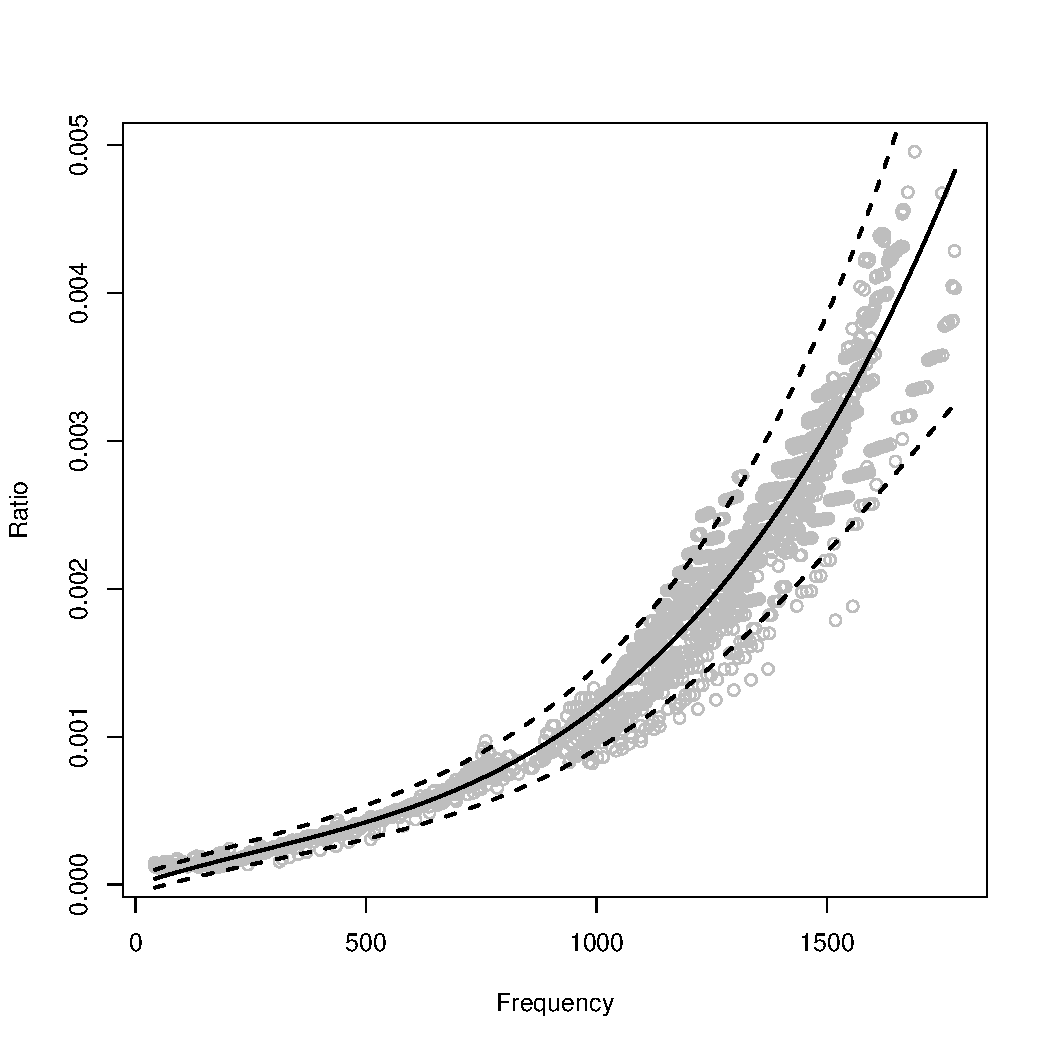
\includegraphics[width=0.5\textwidth,height=0.3\textheight]{plots/model}
 \caption{Data from 25 1D simulations {\sc AENUS-ALCAR } and {\sc CoCoNuT}  code, solid line is the maximum likelihood estimate of heteroscedastic cubic model with 95\% confidence bands.} \label{fig:LMVAR}
\end{figure}

To develop the method we considered the gravitational wave signal
{\tt s20-gw-10kpc} described in Section \ref{sec:simulation}, originally
sampled at 16384 Hz but resampled at 4096 Hz.
A spectrogram of this signal is shown in Figure \ref{fig:spectrogram} based on
autoregressive estimates of the local spectra for successive time intervals of 
\textcolor{red}{length 200} with a \textcolor{red}{ 90\%} overlap.
The dominant emission mode corresponds to the $\mbox{}^2 g_2$-mode and we have
developed a time-frequency method to track the ridge $m(t)$ in the spectrogram,
taking into account that it is monotonically increasing as time goes.
Starting from either the left- or right-most column of the time-frequency matrix
we identify and trace the sequence of amplitude peaks within a certain frequency
band given the monotonicity constraint. Appendix \ref{app:gmode} is providing more
details on the reconstruction of the $g$ mode ridge. 


\begin{figure}
 \centering
 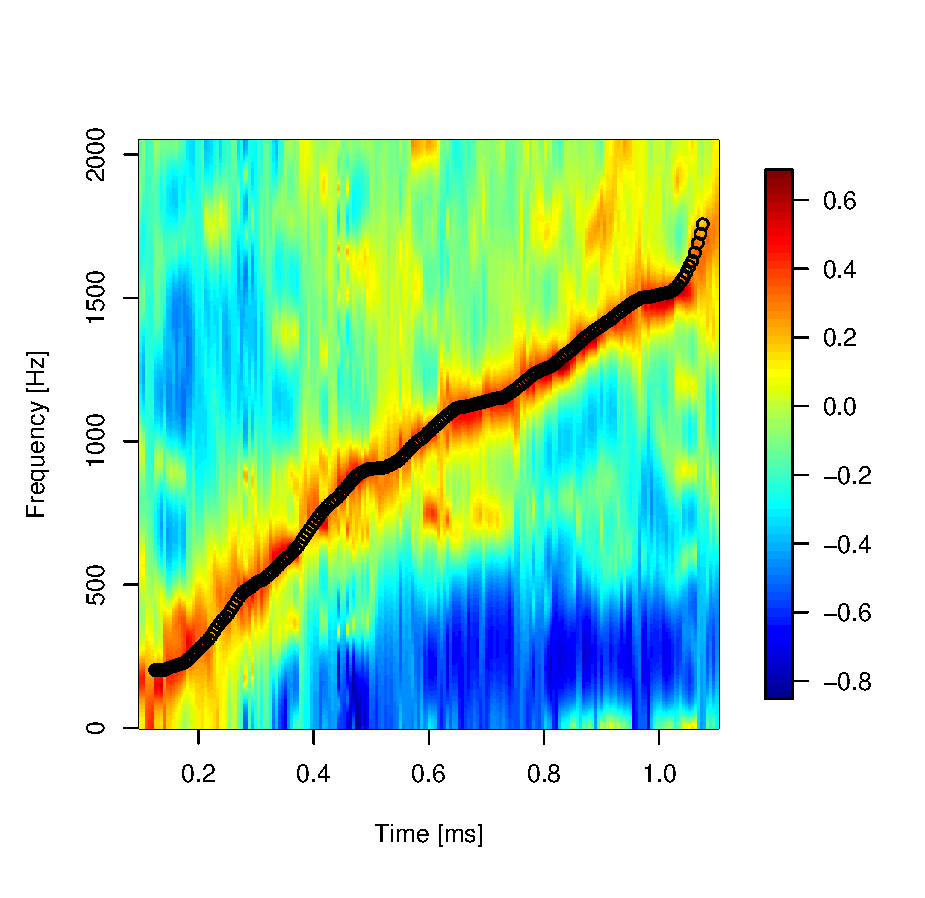
\includegraphics[width=0.5\textwidth,height=0.3\textheight]{plots/spectrogram}
 \caption{Spectrogram of the gravitational wave signal {\tt s20-gw-10kpc} sampled at \unit[4096]{Hz}.
   The spectrogram is obtained using data streach of 200 samples overlapping at 90\%
   with each other.} \label{fig:spectrogram}
\end{figure}


We identify the instantaneous frequency $f(t_i)$ corresponding to the ridge $m(t_i)$ for
the midpoint $t_i$ of each local time interval of the spectrogram and interpolating $f(t)$
for values in between the $t_i$. We then use the equation (\ref{eq:universal}) to obtain
estimates of the time evolution of the ratio together with 95\% confidence intervals.
An exemple is given in Figure \ref{fig:ratio} where the red points are the point estimates and
the grey bands represent 95\% confidence bands. The black points are the true ratio values
computed using the mass and radius values obtained from the simulation code. 

\begin{figure}
 \centering
 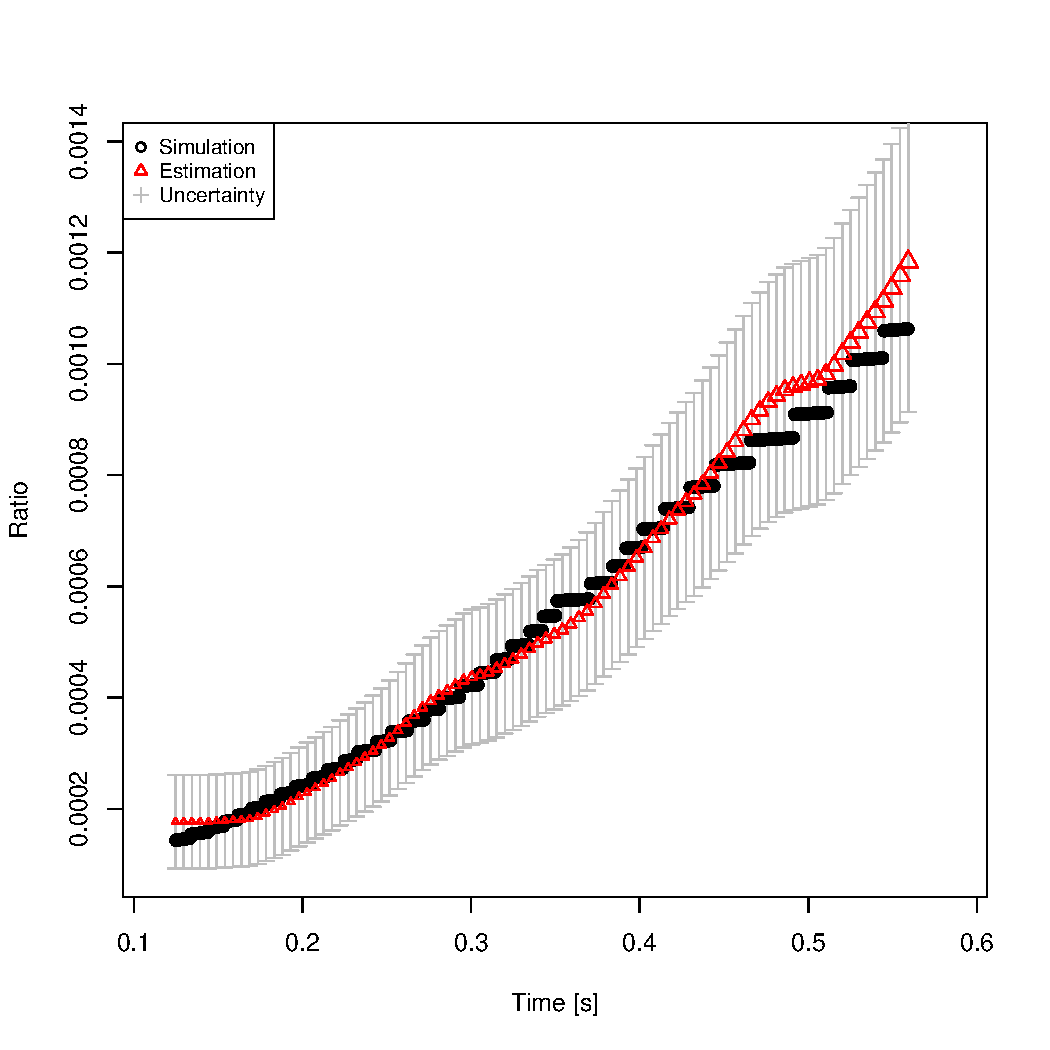
\includegraphics[width=0.5\textwidth,height=0.3\textheight]{plots/ratio}
 \caption{} \label{fig:ratio}
\end{figure}


%In this case without any noise, the coverage of our 95\% confidence band is xx\%.

In the following simulation study we explore how accurately we can estimate the parameters
when the gravitational wave signal is embedded in noise.
For that purpose, we inject the gravitational wave signal into  simulated Advanced LIGO noise
using the noise power spectral density \textcolor{red}{insert formula} for varying
SNRs, respectively distances to the source. We estimate the coverage probability of the 95\%
confidence band by calculating the proportion of times that the true ratio lies outside one
of the pointwise 95\% confidence intervals.
These coverage probabilities together for varying SNRs are given in Table
\textcolor{red}{insert Table} and displayed in the form of boxplots in Figure
\textcolor{red}{insert Figure}





